% !TeX spellcheck = ru_RU
\chapter{Исследовательская часть}

В данном разделе приведены технические характеристики устройства, на котором проводилось измерение времени работы ПО, а также результаты замеров времени.

\section{Технические характеристики}

Ниже приведены технические характеристики устройства, на котором было проведено измерение времени работы ПО:

\begin{itemize}
	\item операционная система Windows 10 Домашняя Версия 21H1 \cite{windows} x86\_64;
	\item оперативная память 8 Гбайт 2133 МГц;
	\item процессор Intel Core i5-8300H с тактовой частотой 2.30 ГГц \cite{intel}, 4 физических ядра, 8 логических ядер.
\end{itemize}

\section{Время выполнения реализации алгоритма}

Для замеров времени использовалась функция получения значения системных часов $clock\_gettime()$ \cite{gettime}. Функция применялась два раза --- в начале и в конце измерения времени, значения полученных временных меток вычитались друг из друга для получения времени выполнения программы.

Документы заполнялись случайными буквами латинского алфавита.
Замеры проводились по 1000 раз для набора значений количества потоков {0, 1, 2, 4, 8, 16, 32, 64}, где значение количества потоков \textit{0} соответствует однопоточной программе, а значение \textit{1} --- программе, создающей один дополнительный поток, выполняющий все вычисления.
В таблице \ref{tbl:threads} представлены замеры времени выполнения программы в зависимости от количества потоков.


\begin{table}[h]
	\begin{center}
		\begin{threeparttable}
			\caption{Результаты нагрузочного тестирования (в мкс)}
			\label{tbl:threads}
			\begin{tabular}{|c|c|c|c|c|c|c|c|c|}
				\hline
				{Кол-во документов} & \multicolumn{8}{c}{Кол-во потоков} \\
				\hline
				 & 0 & 1 & 2 & 4 & 8 & 16 & 32 & 64 \\
				\hline
				2048 & 515 & 761 & 430 & 416 & 525 & 887 & 1674 & 3328 \\
				\hline
				2560 & 648 & 924 & 521 & 462 & 543 & 910 & 1678 & 3339 \\
				\hline
				3072 & 778 & 1066 & 621 & 511 & 590 & 950 & 1730 & 3398 \\
				\hline
				3584 & 927 & 1204 & 700 & 552 & 633 & 984 & 1768 & 3456 \\
				\hline
				4096 & 1042 & 1346 & 809 & 607 & 656 & 1016 & 1807 & 3487 \\
				\hline
				4608 & 1181 & 1484 & 919 & 643 & 706 & 1055 & 1853 & 3493 \\
				\hline
				5120 & 1323 & 1606 & 1016 & 684 & 732 & 1081 & 1862 & 3514 \\
				\hline
				5632 & 1426 & 1738 & 1081 & 734 & 765 & 1104 & 1893 & 3544 \\
				\hline
				6144 & 1571 & 1886 & 1164 & 825 & 816 & 1129 & 1919 & 3598 \\
				\hline
				6656 & 1688 & 2010 & 1247 & 861 & 851 & 1159 & 1953 & 3606 \\
				\hline
				7168 & 1824 & 2135 & 1341 & 968 & 879 & 1249 & 1972 & 3654 \\
				\hline
				7680 & 1954 & 2258 & 1412 & 963 & 937 & 1215 & 1996 & 3666 \\
				\hline
				8192 & 2066 & 2450 & 1504 & 1053 & 956 & 1260 & 2014 & 3711 \\
				\hline
				
			\end{tabular}
		\end{threeparttable}
	\end{center}
\end{table}

%\clearpage
На рисунках \ref{img:nomutex} -- \ref{img:graphic} приведена графическая интерпретация результатов замеров.

\img{0.7}{nomutex}{Результаты замеров времени работы реализаций алгоритма с разным количеством потоков в зависимости от количества документов}
\img{0.7}{graphic}{Результаты замеров времени работы реализации алгоритма для 8192 документов в зависимости от количества потоков}

%\begin{figure}[]
%	\center{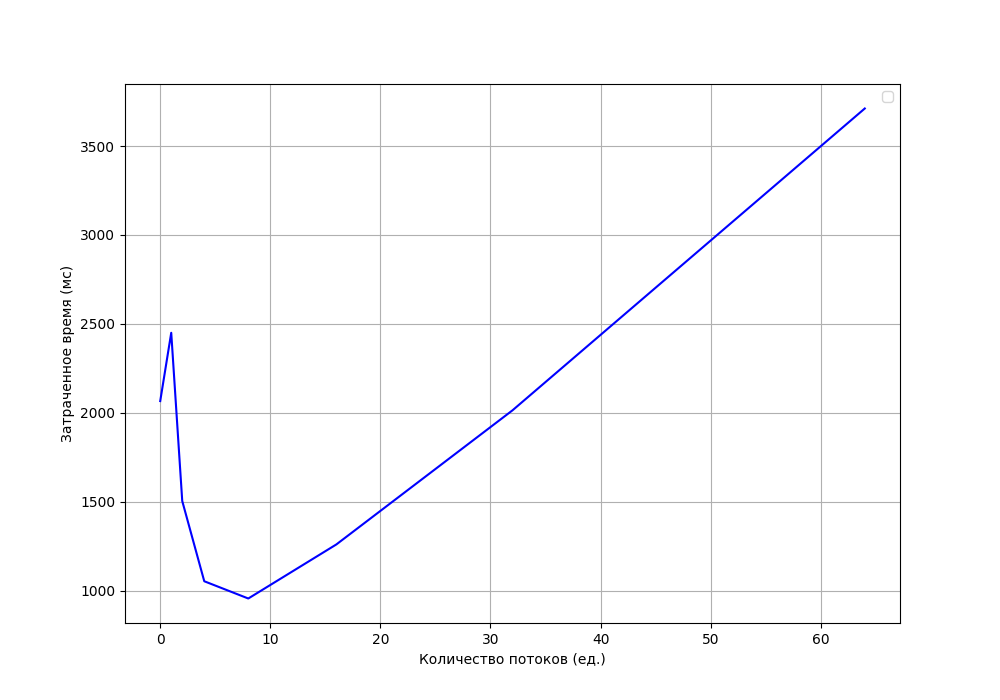
\includegraphics[scale = 0.6]{img/graphic}}
%	\caption{#Результаты замеров времени работы реализации алгоритма для 8192 документов в зависимости от количества потоков}
%	\label{img:#graphic}
%\end{figure}

\clearpage


Из полученных результатов можно сделать вывод, что однопоточный процесс работает быстрее процесса, создающего один отдельный поток для обработки всех документов. Это связано с дополнительными временными затратами на создание потока и передачи ему необходимых аргументов.

Наилучший результат по времени для всех значений количества документов показал процесс с 8 дополнительными потоками, выполняющими вычисления. Рекомендуется использовать на данной архитектуре ЭВМ число дополнительных потоков равное числу логических ядер устройства.

Для числа потоков, большего 8, затраты на содержание потоков превышают преимущество от использования многопоточности, и функция времени от количества потоков начинает расти.

\section*{Вывод}

В результате экспериментов было выявлено, что использование многопоточности может уменьшить время выполнения реализации алгоритма по сравнению с однопоточной программой при условии использования подходящего количества потоков.

Выборка из результатов замеров времени (для 8192 документов):
\begin{itemize}
	\item однопоточный процесс --- 2066 мкс;
	\item один дополнительный поток, выполняющий все вычисления --- 2450 мкс;
	\item 8 потоков (лучший результат) --- 956 мкс, что в 2,16 раз быстрее выполнения однопоточного процесса;
	\item 64 потока (худший результат) --- 3711 мкс, что в 1,80 раз быстрее выполнения однопоточного процесс.
\end{itemize}

Таким образом, использование дополнительных потоков может как ускорить выполнение процесса по сравнению с однопоточным процессом (в 2,16 раз для 8 потоков), так и увеличить время выполнения (в 1,80 раз для 64 потоков).

Рекомендуется использовать на данной архитектуре ЭВМ число дополнительных потоков равное числу логических ядер устройства.


